

\partabstractfp{\textbf{进程第1天课程摘要} }
\partabstractrp{}
\partabstractlettrine{}{} % the first word of the abstract

\part{进程课第1天}

\chapter{进程的代码结构}
\section{进程控制块PCB与task\_struct}
进程是一个资源封装的单位,资源指占用的内存,文件系统,信号及处理方法。线程是调度执行的单元。一个进程区别与另一个进程的标记就是资源。linux操作系统是可以做到进程与进程之间的资源隔离。进程的描述就是资源的描述。PCB (PROCESS CONTROL BLOCK) 在不同操作系统中用于描述进程,在Linux的PCB就是用task\_struct来描述。如\ref{linux_pcb}所示,图中列出了主要对应包含的资源种类及作用。
\begin{figure}[H]
 \wdfigbox
  {\caption{进程控制块PCB}\label{linux_pcb}}
  {
  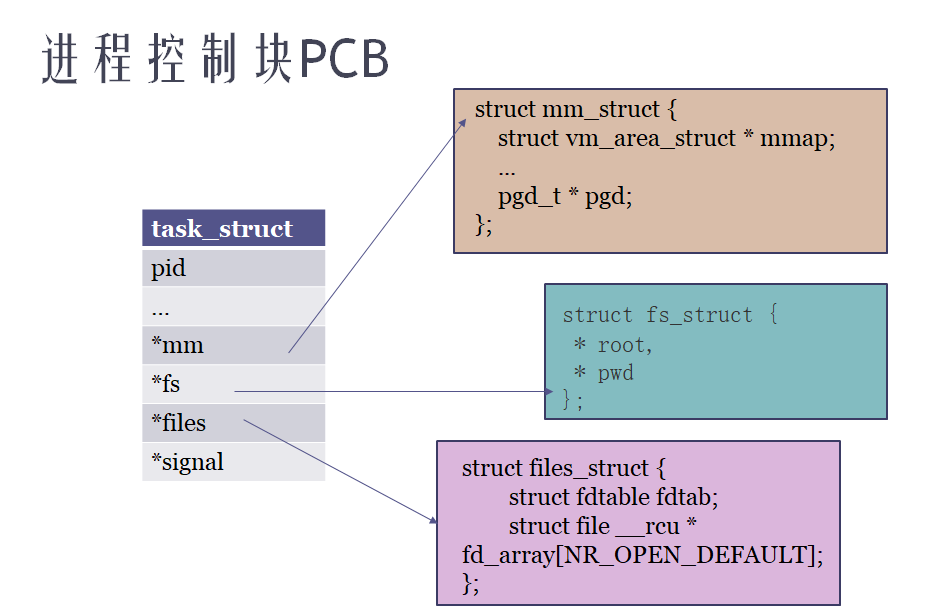
\includegraphics[width=9cm]{./figure/linux_pcb.png}
  \floatfoot{注:即linux中的task\_struct }
  }
\end{figure}
\begin{description}
  \item[\heiti{mm 内存资源:}] 进程的内存
  \item[\heiti{fs 文件系统资源1:}] 根路径和当前路径指针
  \item[\heiti{files 文件系统资源2:}] 进程打开的文件,文件描述符数组
  \item[\heiti{signal 信号资源:}] 不同进程可以针对同一信号挂不同的处理方法
  \item[\heiti{pid 属性资源:}] 描述进程的属性
\end{description}



\section{task\_struct的属性特点}
本节讲的主要是Pid属性是有限的这个特点,利用这个特点,实现linux下破坏死机和代码中破解的例子。
\subsection{fork炸弹让linux死机}
linux下著名的fork炸弹,一敲就让Linux死机。是利用不断利用fork产生进程把pid耗尽,其命令如下:
\begin{example*}
  \wdexpbox
  {\caption{fork炸弹}}
  {linux下著名的fork炸弹,一敲就让Linux死机。\\
  \textcolor[rgb]{1.00,0.00,0.00}{\#linux fork 炸弹}\\  
  \textcolor[rgb]{1.00,0.00,0.00}{\textbf{:()\{:\|:\&\};: } }
  }
\end{example*}

\begin{latexcmd}[label=linux fork 炸弹解析]
: 函数名为冒号

() 函数参数定义

{} 函数定义

:调用自己

|:递归调用自己

& 后台执行

; 函数结束

: 调用函数:
\end{latexcmd}

\subsection{pid数量限制导致安卓的一键root}
安卓的2.2.1之前的版本被发现一个漏洞,很容易就被一键root,安卓的调试软件adb刚开始时有root权限,之后adb调用api setuid(shell) 把自己从root用户降为shell用户。谷歌的工程师在调用时没有检查setuid的返回值,即默认setuid总是可以成功。黑客们利用uid数量有限制的属性,将shell用户内的pid进程全部用完,这样调用setuid时是无法成功的,但因为没有检查返回值,导致adb调用setuid(shell) 后没有降权成功,还是有root权限。这就是Android著名的提权漏洞:rageagainstthecage。2.2之后的安卓版本修复了此漏洞,方法是检查setuid的返回值。

查看Linux中最大Pid数量的命令如下:
\begin{lstlisting}[language={bash}]
wangfan@wangfan-VirtualBox:~$ ulimit -a
core file size          (blocks, -c) 0
data seg size           (kbytes, -d) unlimited
scheduling priority             (-e) 0
file size               (blocks, -f) unlimited
pending signals                 (-i) 15723
max locked memory       (kbytes, -l) 64
max memory size         (kbytes, -m) unlimited
open files                      (-n) 1024
pipe size            (512 bytes, -p) 8
POSIX message queues     (bytes, -q) 819200
real-time priority              (-r) 0
stack size              (kbytes, -s) 8192
cpu time               (seconds, -t) unlimited
max user processes              (-u) 15723
virtual memory          (kbytes, -v) unlimited
file locks                      (-x) unlimited
\end{lstlisting}

\subsection{linux的pid与tgid}
一个进程fork出子进程后,从linux内核的角度看,对应的pid肯定不一样。但是为了符合POSIX的标准要求,POSIX要求规定同一个父进程fork出的子进程,调用getpid返回的pid的号必须是一样的,我们用top命令查看进程可以看到fork出的子进程与父进程的Pid号是一样的。linux实现的原理就是通过增加一个tgid来实现父子进程调用getpid时返回值都一样的效果。
\begin{tcolorbox}[colback=blue!5,colframe=blue!75!black,title=pid和tgid 视频]
\videoattach{4- pid-tgid-pthread-self}{pid和tgid视频演示}
\end{tcolorbox}

\subsection{linux进程task\_struct的三种数据结构}
在linux代码中会涉及各种对task\_struct的引用关系,比如调度算法中会将task\_struct挂在链表上,父子进程的关系用树来描述,CFS调度算法会用到红黑树,通过pid查找进程则是用hash表的结构。其对应的数据结构如\ref{task_datastructure}所示

\begin{figure}[H]
 \wdfigbox
  {\caption{task\_struct汲及到的数据结构}\label{task_datastructure}}
  {
  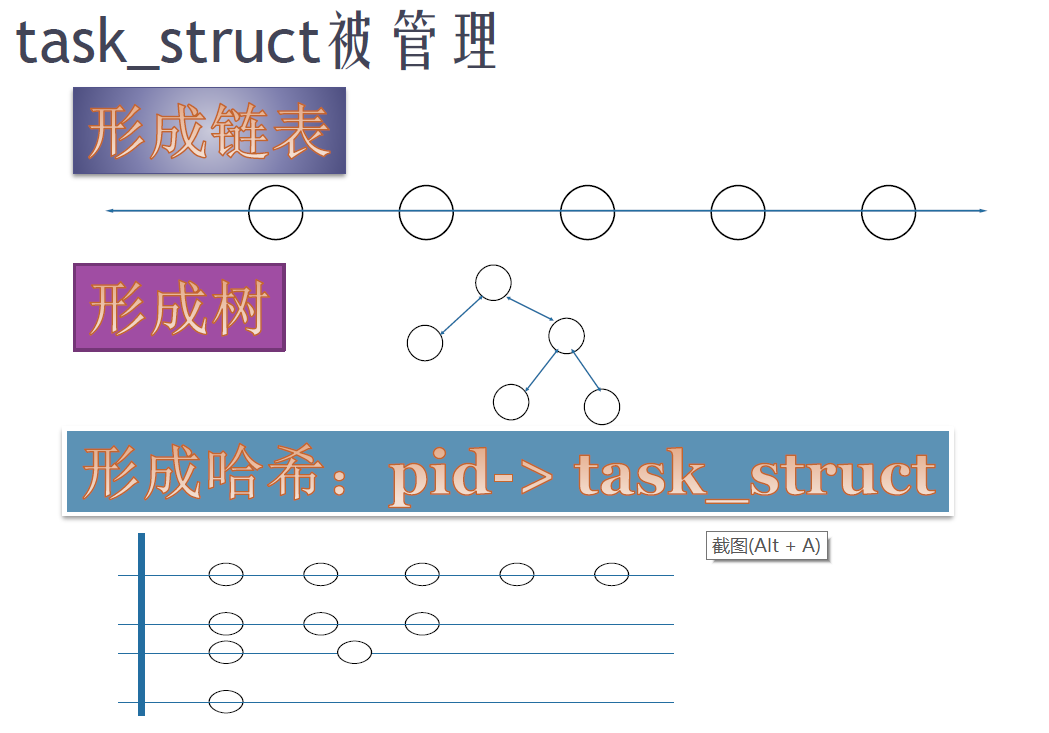
\includegraphics[width=9cm]{./figure/task_datastructure.png}
  \floatfoot{注: 每种数据结构选择都是根据应用场景的需求来选择实现目的效率最高的数据结构}
  }
\end{figure}
\chapter{进程的状态特征}
linux进程的生命周期对应6个状态,
\section{进程状态切换}
\subsection{进程运行时的3个基本状态}
操作系统包括实时系统对应进程一般都有3个状态,进程在有CPU时对应运行态,无CPU时对应就绪态和睡眠态。就绪态指所有资源都准备好,只要有CPU就可以运行了。睡眠指有资源还未准备好,比如读串口数据时,数据还未发送。此时有CPU也无法运行,需要等资源准备好后变成就绪态,然后得到CPU后才能变成运行态,其转换关系如\ref{process_3types}所示。

\begin{figure}[H]
 \wdfigbox
  {\caption{进程基本的三种状态转换}\label{process_3types}}
  {
  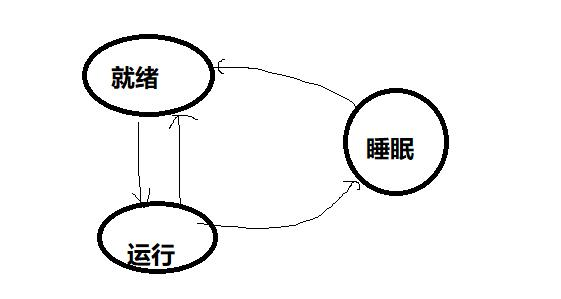
\includegraphics[width=9cm]{./figure/process_3types.jpg}
  \floatfoot{注:linux 除这三种状态外另外增加了状态}
  }
\end{figure}

\subsection{linux进程扩展的6个状态}

\begin{enumerate}
  \item {\heiti{僵尸态:}} 子进程退出后,所有资源都消失了,只剩下task\_struct,父进程在wait函数中可以得到子进程的死亡原因。在wait之前子进程的状态就是僵尸态。
  \item {\heiti{深度睡眠:}} 等待资源到位后才醒过来
  \item {\heiti{浅度睡眠:}} 等待资源到位或收到信号后都会醒过来
  \item  {\heiti{暂停:}} stop状态是被外部命令作业控制等强制进程进入的状态。
  \item  {\heiti{就绪:}} 未占用CPU,等待调度算法调度到运行态的进程
  \item  {\heiti{运行:}} 占有CPU,正在运行的线程。
\end{enumerate}

\begin{figure}[H]
 \wdfigbox
  {\caption{linux 进程6种状态转换}\label{linux_process_6types}}
  {
  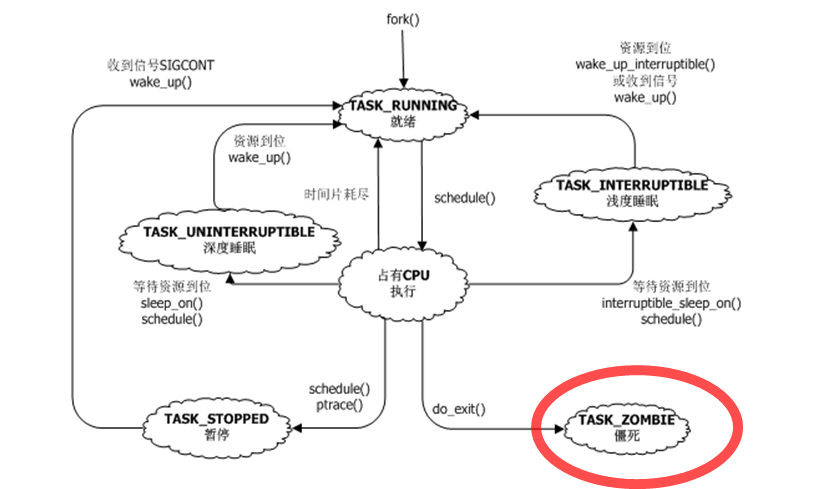
\includegraphics[width=9cm]{./figure/linux_process_6types.png}
  \floatfoot{注:linux 进程的运行转换图}
  }
\end{figure}
暂停状态是进程在运行过程中,通过外部bash命令强制让进程进入的状态。通过这种方法可以指定进程的CPU占用率。后面我们通常用cgroup的方法来实现,这里仅作了解。
\begin{latexcmd}[label=进入stop状态的方法]
作业控制的命令
ctrl + z, fg/bg
cpulimit
cpulimit -l 20 -p 10111
限制pid 为10111程序的CPU使用率不超过20%  
\end{latexcmd}
\subsection{linux进程状态的联系和区别}
\begin{description}
  \item[{\heiti{就绪VS运行}}] linux的调度算法只管理就绪和运行态中的进程,只对应\label{linux_process_6types}中的就绪和占有状态的进程,这两个状态都称为task\_running。
  \item[{\heiti{深度睡眠VS浅度睡眠}}] 深度睡眠只有资源到位才醒,收到信号也不醒,浅度睡眠资源到位或收到信号都会醒
  \item[{\heiti{睡眠VS暂停}}] 睡眠是代码中未得到资源主动进入的状态,暂停是程序外部强制进程进入的状态。
\end{description}


\section{进程的内存泄露}
内存泄露指随着时间的增长,进程的内存使用呈现线性增长的情况,指的是进程一直在运行,运行中申请了内存,但使用完后并没有释放,运行期间每次都申请内存而不释放导致系统内存越来越少的情况。这里要理解内存泄露的原因不可能是进程死了,内存没释放。因为进程死了之后就变成僵尸,Linux会自动将进程中申请的资源全部释放,只留下task\_struct让父进程wait来查看状态。不可能再占用内存。
%%% Local Variables:
%%% TeX-master: "main"
%%% End:
